\documentclass[sigconf,review,anonymous]{acmart}
\usepackage{microtype}
\usepackage{booktabs,multirow,array,xurl}
\usepackage{tikz}
\usetikzlibrary{arrows.meta,positioning,shapes.geometric,fit,calc}
\settopmatter{printfolios=true}
\hypersetup{pdftitle={Encrypted QUIC Application Classification Under Temporal Shift: Full-Population Tree Baselines and a Neural Reference},pdfauthor={}}
\title{Encrypted QUIC Application Classification Under Temporal Shift: Full-Population Tree Baselines and a Neural Reference}
\author{Anonymous Author(s)}
\begin{document}
\begin{abstract}
Encrypted QUIC application classification is challenging because payload inspection is unavailable and traffic distributions evolve. We evaluate a 50-class closed-set task on the medium CESNET-QUICEXT-25 variant with a chronological protocol: 27,727,267 known-class flows from June 2024 through March 2025 for training, disjoint April 2025 partitions for model selection, early stopping, stacking, and calibration audit, and all 2,359,061 known-class flows from May 2025 for testing. The 101-feature representation combines the first 30 packet timing/direction/size triples with 11 auxiliary flow statistics; because some auxiliary features summarize the full flow, this is not strict first-30-packet online classification. LightGBM with an April-trained logistic stacker achieves 0.8789 accuracy and 0.7534 macro-F1, versus 0.8427 and 0.6966 for XGBoost one-vs-rest. A paired bootstrap over 31 test days estimates a 0.0568 macro-F1 advantage (95\% interval 0.0531--0.0607). XGBoost is approximately 4.97 times faster in the measured model-only benchmark. Neural scores are retained only as an external descriptive reference because their checkpoint and per-flow predictions are unavailable.
\end{abstract}
\maketitle
\keywords{QUIC; encrypted traffic classification; temporal generalization; CESNET-QUICEXT-25; LightGBM; XGBoost; one-vs-rest; probability stacking; calibration; day-block bootstrap}



\section{Introduction}
\label{sec:intro}

Encrypted transport is now common across the Internet, and QUIC is a core transport protocol for HTTP/3 and other application traffic. Encryption limits direct access to payload content and to some protocol metadata that traditional port-based identification and deep packet inspection systems used. Yet network management tasks---including traffic characterization, capacity planning, quality-of-service analysis, and security monitoring---still benefit from reliable application-level classification.

A line of encrypted-traffic classification research addresses this challenge by learning from observable side-channel information such as packet sizes, packet direction, inter-packet timing, and flow-level statistics. Such features do not reveal payload content, but may retain statistical regularities associated with application behavior. The challenge is particularly demanding in operational traffic, where application frequencies are highly imbalanced and traffic characteristics can change over time.

This study uses CESNET-QUICEXT-25, a year-long QUIC traffic dataset collected on the CESNET backbone \cite{cesnet-quicext25,waitingforquic}. We analyze two tree-based pipelines under a shared, temporally separated, full-population evaluation protocol and document a previously trained neural stacking ensemble as an external reference. The primary research question is how the tree pipelines compare under this protocol; the missing neural checkpoint and per-flow predictions limit the strength of cross-family claims.

The study makes five contributions:
\begin{itemize}
  \item We report results on a 50-class closed-set task using 27.7 million training flows and the complete 2.36 million-flow May 2025 test population.
  \item We compare multiclass LightGBM with an XGBoost one-vs-rest (OvR) ensemble under a common 101-feature representation, disjoint April development partitions, and a complete May test population.
  \item We reconstruct and document the previously trained neural stacking\_A\_C architecture from its supplied notebook while explicitly separating descriptive reference scores from controlled tree-family inference.
  \item We report aggregate metrics, 95\% bootstrap confidence intervals, per-class F1 scores, calibration error, and model-only inference benchmarks.
  \item We document the implementation and interpretation boundaries of the comparison, including the non-native multiclass formulation used for XGBoost, the distinction between matching data populations and matching compute budgets, and the limitations of a single held-out month.
\end{itemize}

\section{Related Work}
\label{sec:related}

Encrypted traffic classification has evolved from port-based rules and payload inspection toward statistical machine learning and deep learning over packet sequences and flow summaries. This shift is driven by encryption's reduction of visible payload information, but classification remains sensitive to dataset construction, label granularity, traffic drift, and whether evaluation separates future traffic from the training period. Surveys by Rezaei and Liu and by Sharma and Lashkari review deep-learning and broader encrypted-traffic classification methods, respectively \cite{rezaei2019,sharma2025survey}. These surveys also motivate evaluating more than accuracy alone, particularly when class imbalance and operational constraints matter.

QUIC-specific studies span different tasks and data regimes. Earlier ensemble-based QUIC classification evaluated a small set of application/service categories, while VisQUIC provides more than 100,000 labeled traces from over 40,000 websites and studies encrypted QUIC dynamics, including request--response estimation \cite{quicensemble2023,visquic2024}. CESNET-QUICEXT-25 instead provides a year-long backbone dataset with extended attributes; the present study uses its medium variant for 50-class application classification and evaluates on a complete later calendar month \cite{cesnet-quicext25,waitingforquic}. These datasets and tasks are complementary rather than directly interchangeable: label definitions, collection environments, feature availability, and split strategies differ.

Our model families also reflect distinct inductive biases. LightGBM is a gradient-boosted decision-tree method designed for efficient large-scale training \cite{lightgbm}; XGBoost is a scalable tree-boosting framework, here used in a one-vs-rest decomposition because the native multiclass configuration was not feasible under the run's GPU-memory constraints \cite{xgboost}. The external neural reference combines squeeze-and-excitation residual convolutional blocks, which adaptively reweight channels, with Transformer self-attention for sequence representation \cite{hu2018senet,vaswani2017attention}. The main contribution here is not a new architecture: it is a full-population, temporally separated comparison of two tree pipelines, paired day-block uncertainty estimates, an April-only stacking/calibration protocol, and an explicit account of what the available artifacts do and do not support about the external neural reference.

\section{Dataset and Task}
\label{sec:dataset}

\subsection{Dataset and label space}

CESNET-QUICEXT-25 covers twelve consecutive months, from June 2024 through May 2025, and is distributed in multiple size variants through \texttt{cesnet-datazoo}. We use the medium (M) variant. The underlying HDF5 database contains 50 million rows across 360 daily flow tables. The task uses the \texttt{ALL\_KNOWN} closed-set label space of 50 application classes; the two background labels identified in the data schema are excluded. Results therefore describe classification among these 50 known classes, not open-set recognition of arbitrary unseen or background traffic.

The dataset applies uniform 1:100 flow sampling without per-application rebalancing, according to the dataset description. The class distribution is consequently highly skewed. The exact number of rows retained for this experiment depends on the known-class policy and the temporal partition, rather than being equal to the raw 50-million-row database size.

\subsection{Features}

Each flow is represented by 101 numerical features:
\begin{itemize}
  \item \textbf{Per-packet information (90 features):} the first 30 packets, each represented by inter-packet time (IPT), direction (DIR), and packet size (SIZE).
  \item \textbf{Auxiliary flow statistics (11 features):} \texttt{BYTES}, \texttt{BYTES\_REV}, \texttt{PACKETS}, \texttt{PACKETS\_REV}, \texttt{DURATION}, three flow-end-reason indicators, \texttt{PPI\_DURATION}, \texttt{PPI\_LEN}, and \texttt{PPI\_ROUNDTRIPS}.
\end{itemize}
No payload bytes or SNI feature is used by the evaluated 101-dimensional representation. An important scope distinction is that some auxiliary statistics describe the full flow. The experiment should therefore be understood as flow-level classification with an early-packet sequence component, not as a strict online classifier that makes a decision from the first 30 packets alone.

\begin{table*}[t]
\centering
\caption{Input representation used by the tree pipelines and neural reference.}
\label{tab:feature_schema}
\small
\begin{tabular}{p{0.23\textwidth}p{0.20\textwidth}p{0.45\textwidth}}
\toprule
Feature group & Shape & Contents / interpretation \\
\midrule
Packet sequence & $30\times3$ & 30 positions; each contains inter-packet time (IPT), direction (DIR), and packet size (SIZE). \\
Auxiliary flow statistics & $11$ & Bytes and packets in both directions, duration, three end-reason indicators, and PPI duration/length/roundtrips. \\
Tree input & $101$ & Flattened packet fields plus auxiliary features. \\
Neural input & Two inputs & Sequence tensor $30\times3$ and a separate 11-dimensional auxiliary vector. \\
\bottomrule
\end{tabular}
\end{table*}

\subsection{Chronological data partition}

The partition is chronological, with non-overlapping periods:
\begin{itemize}
  \item \textbf{Training:} 1 June 2024--31 March 2025 (299 days), containing 27{,}727{,}267 known-class flows. No training-row subsampling was used for the tree baselines.
  \item \textbf{April development reservoir:} 1--30 April 2025, containing 600{,}000 known-class flows split by a deterministic permutation into disjoint subsets of 30{,}000 for HPO validation, 70{,}000 for early stopping, 400{,}000 for probability-stacker fitting, and 100{,}000 for a calibration audit.
  \item \textbf{Test:} 1--31 May 2025, containing all 2{,}359{,}061 known-class test flows.
\end{itemize}

The chronological design tests generalization to later traffic rather than randomly interleaving flows from the same time period. The April partitions serve separate development roles; the 100,000-row audit is not used for selection. May remains untouched until both tree models and stackers are frozen. The test results measure performance on one subsequent month; they do not establish robustness to longer-term drift across multiple future months.

\begin{table*}[t]
\centering
\caption{Chronological data protocol and partition roles.}
\label{tab:split}
\small
\begin{tabular}{p{0.22\textwidth}p{0.25\textwidth}rp{0.32\textwidth}}
\toprule
Partition & Period & Flows & Permitted use \\
\midrule
Training & Jun. 2024--Mar. 2025 & 27,727,267 & Fit preprocessing, class weights, and tree models \\
HPO & Apr. 2025 & 30,000 & Hyperparameter selection \\
Early stopping & Apr. 2025 & 70,000 & Tree iteration selection \\
Stacker fitting & Apr. 2025 & 400,000 & Fit multinomial logistic stackers \\
Calibration audit & Apr. 2025 & 100,000 & Post-selection calibration audit only \\
Final test & May 2025 & 2,359,061 & Single frozen full-population evaluation \\
\bottomrule
\end{tabular}
\end{table*}

\section{Preprocessing and Models}
\label{sec:method}

\subsection{Preprocessing}

The preprocessing pipeline is fitted on the training period only. Non-negative timing, size, and auxiliary continuous values are clipped at zero and transformed using $\log(1+x)$ before standardization. The direction channel is retained without standardization. The scaler statistics are accumulated over the training population in chunks rather than being estimated from a small random subset.

Flows with fewer than 30 observed packets are padded. Since a standard scaler would map padded zeros to nonzero standardized values, the implementation uses the direction channel to identify padding and restores the corresponding timing and size entries to zero after transformation. This preserves the distinction between an absent packet and a measured packet with a small value. The same fitted preprocessing object is applied to validation and test data; no test statistics are used to fit it.

This preprocessing differs from the stock clipping-and-scaling transform supplied with \texttt{cesnet-models}. Results should therefore be compared directly only with baselines using the same representation and preprocessing, or with published results whose preprocessing is explicitly reconciled.

\subsection{Class imbalance}

The known-class distribution is highly imbalanced. The tree baselines use sample weights derived from inverse training-class frequency, normalized to have mean one and clipped to the interval $[0.25,5.0]$. The weights are calculated from training labels only. No test-set label information is used to derive class weights.

The neural reference was trained in a separate experiment and is treated here as a fixed reference model. Its training configuration, including its loss and imbalance handling, is not re-optimized as part of the tree-baseline experiment. Accordingly, matching the training population and feature visibility does not mean that the models use identical objective functions or optimization budgets.

\subsection{Neural reference: architecture and provenance}
\label{sec:neural}

The external neural reference is the \texttt{stacking\_A\_C} ensemble produced by the supplied Pass 3 notebook. Four candidate sequence architectures were defined in that notebook, but the April validation-selection procedure retained only Model A and Model C and selected logistic-regression stacking of their 50-class probability vectors. The architecture description below is reconstructed from the supplied notebook source and recorded hyperparameters; the Pass 5 ZIP does not include the trained neural weights/checkpoint or per-flow neural probabilities.

\begin{table*}[t]
\centering
\caption{Neural reference at a glance. These details describe the notebook-defined architecture, not a newly retrained Pass 5 model.}
\label{tab:neural_overview}
\small
\begin{tabular}{p{0.22\textwidth}p{0.31\textwidth}p{0.34\textwidth}}
\toprule
Component & Model A: SE-ResNet1D & Model C: lightweight Transformer \\
\midrule
Sequence input & $30\times3$ & $30\times3$ \\
Sequence encoder & 3 residual Conv1D blocks; 96/192/384 channels & Dense projection to 96; 3 encoder blocks \\
Context mechanism & Local convolution + channel-wise SE gates & 8-head self-attention; 12 key dimensions/head \\
Pooling & Global average + global max & Global average + global max \\
Auxiliary branch & 11 features $\to$ Dense(64) & 11 features $\to$ Dense(64) \\
Dense classifier head & 256 $\to$ 128 $\to$ softmax(50) & 256 $\to$ 64 $\to$ softmax(50) \\
Selected activation & GELU & Swish \\
\bottomrule
\end{tabular}
\end{table*}

\begin{figure*}[t]
\centering
\resizebox{0.98\textwidth}{!}{%
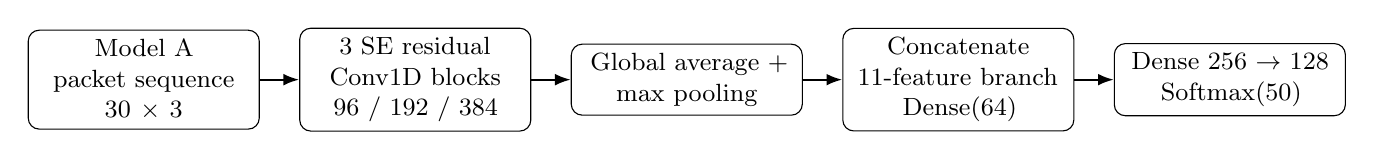
\begin{tikzpicture}[
  box/.style={draw,rounded corners,align=center,minimum height=8mm,text width=27mm,font=\small},
  arr/.style={-{Latex[length=2mm]},thick},
  node distance=5mm
]
\node[box] (a) {Model A\\packet sequence\\$30\times3$};
\node[box,right=of a] (acnn) {3 SE residual\\Conv1D blocks\\96 / 192 / 384};
\node[box,right=of acnn] (apool) {Global average +\\max pooling};
\node[box,right=of apool] (aaux) {Concatenate\\11-feature branch\\Dense(64)};
\node[box,right=of aaux] (ahead) {Dense 256 $\to$ 128\\Softmax(50)};
\draw[arr] (a)--(acnn); \draw[arr] (acnn)--(apool); \draw[arr] (apool)--(aaux); \draw[arr] (aaux)--(ahead);
\end{tikzpicture}}
\caption{Model A: squeeze-and-excitation residual one-dimensional CNN. The first two blocks are followed by max-pooling; each block contains two convolutions, batch normalization, a residual shortcut, and an SE channel gate.}
\label{fig:model_a}
\end{figure*}

\begin{figure*}[t]
\centering
\resizebox{0.98\textwidth}{!}{%
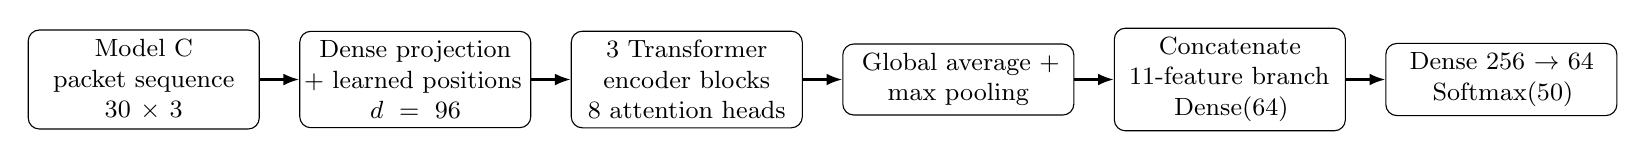
\begin{tikzpicture}[
  box/.style={draw,rounded corners,align=center,minimum height=8mm,text width=27mm,font=\small},
  arr/.style={-{Latex[length=2mm]},thick},
  node distance=5mm
]
\node[box] (c) {Model C\\packet sequence\\$30\times3$};
\node[box,right=of c] (proj) {Dense projection\\+ learned positions\\$d=96$};
\node[box,right=of proj] (enc) {3 Transformer\\encoder blocks\\8 attention heads};
\node[box,right=of enc] (cpool) {Global average +\\max pooling};
\node[box,right=of cpool] (caux) {Concatenate\\11-feature branch\\Dense(64)};
\node[box,right=of caux] (chead) {Dense 256 $\to$ 64\\Softmax(50)};
\draw[arr] (c)--(proj); \draw[arr] (proj)--(enc); \draw[arr] (enc)--(cpool); \draw[arr] (cpool)--(caux); \draw[arr] (caux)--(chead);
\end{tikzpicture}}
\caption{Model C: lightweight Transformer encoder. Each encoder block uses multi-head self-attention and a position-wise feed-forward network, with residual connections, dropout, and layer normalization.}
\label{fig:model_c}
\end{figure*}

\paragraph{Model A: squeeze-and-excitation residual 1D CNN.}
The packet input is a $30\times3$ tensor containing inter-packet time, direction, and packet size. Model A applies three residual 1D convolutional blocks with kernel width 3 and channel widths 96, 192, and 384. Each block contains a same-padded convolution, batch normalization, GELU activation, spatial dropout (rate 0.2159), a second same-padded convolution and batch normalization, and a squeeze-and-excitation gate. The gate globally averages each channel, maps the channel descriptor through a ReLU bottleneck of width approximately one eighth of the channel count (minimum width four), and uses a sigmoid projection to rescale the feature maps. A 1D convolutional projection aligns residual dimensions when the channel width changes. Max-pooling by two is applied after the first two blocks. Global average and global max pooling are concatenated to form the packet-sequence representation.

\paragraph{Model C: lightweight Transformer encoder.}
Model C projects each of the 30 packet tokens to $d_{\mathrm{model}}=96$, adds a learned trainable positional embedding, and applies three Transformer encoder blocks. Each block uses eight-head self-attention with key dimension 12 per head, dropout, residual connections, and layer normalization, followed by a position-wise feed-forward network of width 192 ($2d_{\mathrm{model}}$), swish activation, dropout, a residual connection, and layer normalization. Global average and max pooling are concatenated to obtain the packet-sequence representation.

\paragraph{Shared auxiliary branch and classifier heads.}
Both models take the same 11 auxiliary flow-statistics features through a parallel dense branch (64 units, GELU for Model A or swish for Model C, batch normalization, and dropout 0.2). The branch is concatenated with the pooled packet representation. Model A uses a two-layer dense head with 256 and 128 units; Model C uses 256 and 64 units. Each head layer is preceded by dropout at the model-specific tuned rate and followed by batch normalization; a 50-unit softmax layer produces class probabilities. The selected Model A settings were GELU, dropout 0.2159, focal-loss $\gamma=1.0698$, label smoothing 0.0427, Adam, and peak learning rate $1.558\times10^{-3}$. Model C used swish, dropout 0.1697, focal-loss $\gamma=1.1046$, label smoothing 0.00931, Adam, and peak learning rate $9.438\times10^{-4}$. The notebook defines a warm-up/cosine learning-rate schedule, gradient clipping at norm 1, and a weighted focal loss; early stopping monitors April validation macro-F1 (patience eight) and restores the best weights. The recorded full-training run allowed up to 15 epochs per finalist.

\paragraph{Stacking procedure and evidential status.}
On April, the notebook split a 500,000-flow selection sample into stratified halves to compare individual models, uniform/weighted averaging, and logistic-regression stacking. Stacking used concatenated Model A and Model C probability vectors (100 inputs for 50 classes per model), with logistic regression ($C=0.5$, LBFGS, up to 300 iterations). It was selected using the validation holdout and then refit on the complete 500,000-flow selection sample. The supplied notebook's printed May report gives accuracy 0.9324, macro-precision 0.8725, macro-recall 0.8272, macro-F1 0.8386, weighted-F1 0.9320, and 10-bin ECE 0.0096; these rounded values match the external summary. Nevertheless, Pass 5 records a provenance warning, and the uploaded experiment archive lacks the neural checkpoint and per-flow probability/prediction arrays needed to independently recompute those results or perform a paired day-block bootstrap. The neural scores are therefore presented descriptively, without a neural confidence interval or an inferential claim against the tree models. Its separate notebook benchmark is also excluded from the Pass 5 tree-throughput comparison because the benchmark artifacts and inference path are not shared.

\begin{figure*}[t]
\centering
\resizebox{0.96\textwidth}{!}{%
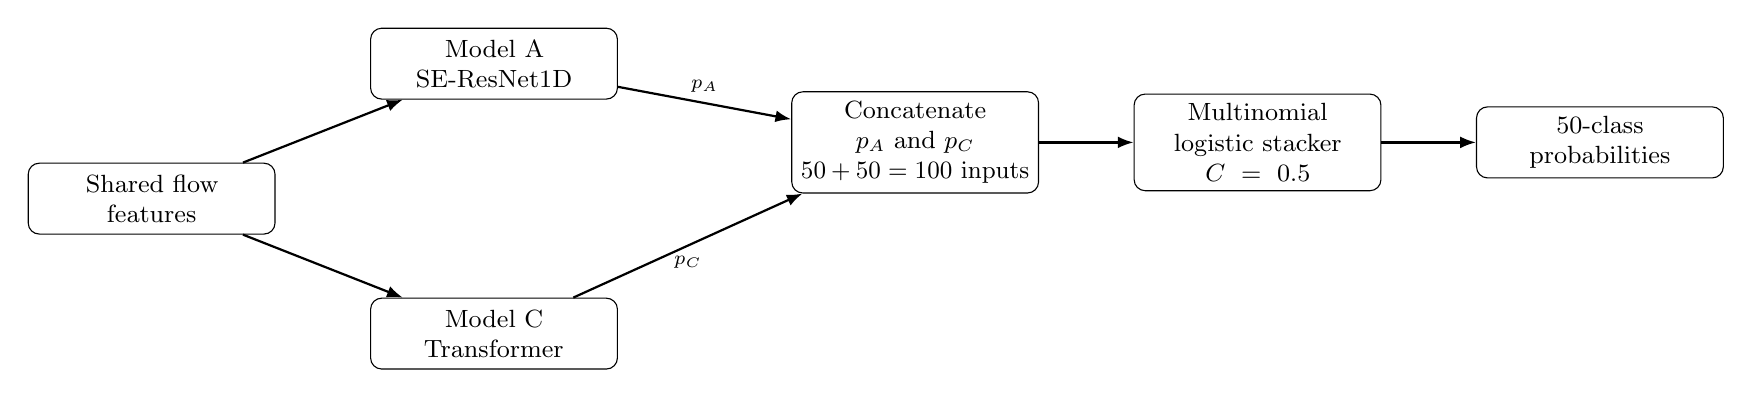
\begin{tikzpicture}[
  box/.style={draw,rounded corners,align=center,minimum height=9mm,text width=29mm,font=\small},
  arr/.style={-{Latex[length=2mm]},thick},
  node distance=8mm and 12mm
]
\node[box] (input) {Shared flow\\features};
\node[box,above right=of input] (modela) {Model A\\SE-ResNet1D};
\node[box,below right=of input] (modelc) {Model C\\Transformer};
\node[box,right=22mm of modela,yshift=-10mm] (concat) {Concatenate\\$p_A$ and $p_C$\\$50+50=100$ inputs};
\node[box,right=of concat] (lr) {Multinomial\\logistic stacker\\$C=0.5$};
\node[box,right=of lr] (out) {50-class\\probabilities};
\draw[arr] (input)--(modela); \draw[arr] (input)--(modelc);
\draw[arr] (modela)--node[above,font=\scriptsize]{$p_A$}(concat);
\draw[arr] (modelc)--node[below,font=\scriptsize]{$p_C$}(concat);
\draw[arr] (concat)--(lr); \draw[arr] (lr)--(out);
\end{tikzpicture}}
\caption{The external \texttt{stacking\_A\_C} prediction path reconstructed from Pass 3. The meta-classifier receives concatenated class-probability vectors; this figure describes the notebook architecture and does not imply that the neural checkpoint or raw predictions were available in Pass 5.}
\label{fig:neural_stack}
\end{figure*}

\begin{table}[t]
\centering
\caption{Selected neural training settings recorded in Pass 3.}
\label{tab:neural_training}
\small
\begin{tabular}{lrr}
\toprule
Setting & Model A & Model C \\
\midrule
Dropout rate & 0.2159 & 0.1697 \\
Focal-loss $\gamma$ & 1.0698 & 1.1046 \\
Label smoothing & 0.0427 & 0.00931 \\
Peak learning rate & $1.558\times10^{-3}$ & $9.438\times10^{-4}$ \\
Optimizer & Adam & Adam \\
Gradient clipping norm & 1.0 & 1.0 \\
Maximum epochs & 15 & 15 \\
Early-stopping patience & 8 & 8 \\
Stacker input width & 100 & 100 \\
\bottomrule
\end{tabular}
\end{table}

\subsection{LightGBM baseline}

LightGBM uses the native 50-class multiclass objective. Hyperparameter search completed four trials on a fixed 100,000-row pilot set and selected learning rate 0.05, 63 leaves, minimum child samples 100, maximum bin count 31, $L_2$ regularization 1.0, row subsampling 0.9, and column subsampling 0.8. The final configuration uses GPU training with double precision for histogram accumulation, seed 20261003, and training-derived class weights. The final iteration cap was 260 with early-stopping patience 35; the recorded best iteration is 260, so the model reached its cap. This is a cap hit, not evidence that the optimization had converged. The run records 25,361.7 seconds for final fitting.

\subsection{XGBoost one-vs-rest baseline}
\label{sec:models}

XGBoost is implemented as 50 independent binary \texttt{binary:logistic} classifiers, one per class, because the native multiclass path exceeded the available GPU memory in earlier attempts. Hyperparameter search completed six trials and selected learning rate 0.1, maximum depth 5, \texttt{min\_child\_weight}=10, 64 histogram bins, $L_1$ regularization 0.1, $L_2$ regularization 1.0, row subsampling 0.9, and column subsampling 0.8. Training uses CUDA and external-memory data access. Each binary classifier uses up to 209 boosting rounds with early-stopping patience 25. The recorded best iteration is 208 overall and nearly all per-class models stop at or near the 209-round cap; consequently, convergence before the iteration limit is not established. Final fitting took 12,091.7 seconds.

At inference, the 50 positive-class sigmoid outputs are concatenated and row-normalized to produce a 50-class score vector before the same multinomial logistic stacking procedure used for LightGBM. Row-normalization is a score-coupling heuristic; it does not make the independently trained binary models equivalent to a jointly optimized \texttt{multi:softprob} model. XGBoost-OvR is therefore interpreted as a separate baseline formulation.

\begin{table*}[t]
\centering
\caption{Final tree-model configurations and optimization limits.}
\label{tab:tree_config}
\small
\begin{tabular}{p{0.25\textwidth}p{0.29\textwidth}p{0.29\textwidth}}
\toprule
Setting & LightGBM & XGBoost-OvR \\
\midrule
Objective & 50-class multiclass & 50 binary logistic models \\
Learning rate & 0.05 & 0.1 \\
Tree complexity & 63 leaves & Depth 5 \\
Minimum child constraint & 100 samples & Weight 10 \\
Histogram bins & 31 & 64 \\
Regularization & $L_2=1.0$ & $L_1=0.1$, $L_2=1.0$ \\
Row / feature sampling & 0.9 / 0.8 & 0.9 / n.a. \\
Iteration cap & 260 & 209 per class \\
Early-stopping patience & 35 & 25 \\
Observed stopping & Best iteration 260 (cap hit) & Most models at/near cap \\
\bottomrule
\end{tabular}
\end{table*}

\begin{figure*}[t]
\centering
\resizebox{0.96\textwidth}{!}{%
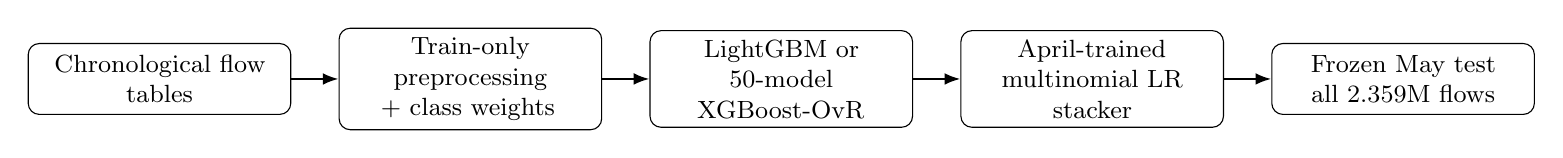
\begin{tikzpicture}[
  box/.style={draw,rounded corners,align=center,minimum height=9mm,text width=31mm,font=\small},
  arr/.style={-{Latex[length=2mm]},thick},
  node distance=6mm
]
\node[box] (raw) {Chronological flow\\tables};
\node[box,right=of raw] (feat) {Train-only\\preprocessing\\+ class weights};
\node[box,right=of feat] (tree) {LightGBM or\\50-model XGBoost-OvR};
\node[box,right=of tree] (stack) {April-trained\\multinomial LR\\stacker};
\node[box,right=of stack] (test) {Frozen May test\\all 2.359M flows};
\draw[arr] (raw)--(feat); \draw[arr] (feat)--(tree); \draw[arr] (tree)--(stack); \draw[arr] (stack)--(test);
\end{tikzpicture}}
\caption{Pass 5 evaluation pipeline. April data is partitioned by role; the calibration-audit subset is held out from selection, and the May population is evaluated only after tree models and stackers are frozen.}
\label{fig:pass5_pipeline}
\end{figure*}

\subsection{Validation and test protocol}

The 600,000-row April reservoir is divided by a single deterministic permutation into four non-overlapping partitions: 30,000 rows for HPO selection, 70,000 for final-model early stopping, 400,000 for fitting the tree probability stackers, and 100,000 for a calibration audit. The manifest records these partitions as disjoint. Both tree families use the same partitions and the same multinomial logistic-regression stacker recipe ($C=1$, LBFGS, maximum 250 iterations); the calibration-audit partition is not used for model or stacker selection. May is held out until the tree models and stackers are frozen, and the final evaluation uses all 2,359,061 known-class flows. The evaluation is thus a chronological, full-population test for May 2025, not an evaluation over multiple future months.

\section{Experimental Setup}
\label{sec:setup}

\subsection{Implementation and hardware}

The final Pass 5 v10 run used Kaggle with two NVIDIA Tesla T4 GPUs. The recorded libraries were NumPy 2.1.3, Pandas 2.3.3, scikit-learn 1.6.1, LightGBM 4.6.0, XGBoost 3.4.1, joblib 1.6.0, and PyTables 3.10.2. The final manifest reports approximately 31.35 GiB of system RAM and 40,931.8 seconds of total wall-clock runtime (about 11.4 hours); the run log reports a similar duration. This end-to-end time includes data preparation, hyperparameter search, fitting, evaluation, and report generation and is not a direct model-efficiency comparison.

\subsection{Metrics}

We report accuracy, macro-averaged precision, macro-averaged recall, macro-F1, support-weighted F1, and 10-bin expected calibration error (ECE). Macro-F1 gives equal weight to each class, while weighted-F1 weights each class by its test support. ECE is computed by binning maximum predicted confidence into ten equal-width confidence bins and taking the support-weighted absolute difference between mean confidence and empirical accuracy. Lower ECE indicates better calibration under this specific binning definition.

Inference throughput is measured at batch size 512 after five warm-up batches and 50 measured batches. For both tree pipelines, the scope includes tree prediction plus the April-trained multinomial logistic stacker; preprocessing and HDF5 I/O are excluded. The XGBoost measurement includes all 50 binary boosters and row normalization. Throughput is therefore a model-stack microbenchmark, not end-to-end application throughput. The neural notebook reports a separate benchmark, but it is not included in the tree comparison because the Pass 5 artifacts do not establish a shared benchmark path.

\subsection{Uncertainty estimates}

The tree-family confidence intervals use 1,000 bootstrap replicates over the 31 May calendar-day blocks. Each replicate samples day blocks with replacement; the same sampled day indices are used for LightGBM and XGBoost, making their metric differences paired at the day-block level. The paired difference is calculated as LightGBM minus XGBoost-OvR. These intervals quantify variation across the observed days within this one month; they do not quantify between-month or between-network uncertainty. No neural bootstrap interval is reported because the Pass 5 archive does not contain neural per-flow predictions or per-day confusion matrices. The manifest records seed 20261006 for the bootstrap procedure.

\section{Results}
\label{sec:results}

\subsection{Aggregate test performance}

Table~\ref{tab:overall} reports the complete May 2025 known-class population. The neural result is included only as an external descriptive reference from the Pass 3 notebook; the controlled and inferential comparison in Pass 5 is between the two tree pipelines.

\begin{table*}[t]
\centering
\caption{May 2025 full-population test results ($N=2{,}359{,}061$). Neural results are external point estimates and are not inferentially compared with the tree rows. Tree throughput includes the April-trained logistic stacker but excludes preprocessing and HDF5 I/O.}
\label{tab:overall}
\resizebox{\textwidth}{!}{%
\begin{tabular}{lrrrrrrr}
\toprule
Model & Accuracy & Macro-P & Macro-R & Macro-F1 & Weighted-F1 & ECE$_{10}$ & Throughput (flows/s)\\
\midrule
Neural stacking\_A\_C (external) & 0.9324 & 0.8725 & 0.8272 & 0.8386 & 0.9320 & 0.0096 & --\\
LightGBM + April LR stacker & 0.8789 & 0.8144 & 0.7275 & \textbf{0.7534} & 0.8774 & 0.0154 & 1{,}254.7\\
XGBoost-OvR + April LR stacker & 0.8427 & 0.7716 & 0.6642 & 0.6966 & 0.8400 & 0.0141 & \textbf{6{,}235.5}\\
\bottomrule
\end{tabular}}
\end{table*}

Among the two controlled tree pipelines, LightGBM exceeds XGBoost-OvR by 3.62 percentage points in accuracy, 4.28 points in macro-precision, 6.32 points in macro-recall, 5.68 points in macro-F1, and 3.74 points in weighted-F1. The paired day-block bootstrap intervals for these differences all exclude zero (Table~\ref{tab:diff}); the inference is specifically about the sampled daily blocks within May 2025. XGBoost-OvR is faster in the model-only benchmark: 6,235.5 versus 1,254.7 flows/s, or approximately 4.97 times the measured throughput. This is a trade-off between stronger class-balanced performance for LightGBM and faster inference for XGBoost-OvR under the benchmark's restricted scope.

The neural reference has higher reported point estimates than either tree model, but that gap is not presented as a controlled inferential result. Although the supplied Pass 3 notebook prints the same rounded aggregate neural scores as the external summary, the Pass 5 manifest retains a provenance warning and the uploaded archive does not include the neural checkpoint or raw per-flow probabilities. It is therefore not possible from the provided artifacts to independently recompute the neural scores or calculate a paired neural-versus-tree day-block interval.

\subsection{Bootstrap intervals for tree baselines}

Table~\ref{tab:ci} reports the 95\% day-block bootstrap intervals for macro-F1. The interval for LightGBM is 0.7471--0.7606; for XGBoost-OvR it is 0.6911--0.7020. The paired difference interval is 0.0531--0.0607, supporting a positive LightGBM advantage for this test month under the specified block-resampling procedure.

\begin{table}[t]
\centering
\caption{Macro-F1 and 95\% paired day-block bootstrap confidence intervals.}
\label{tab:ci}
\begin{tabular}{lrrr}
\toprule
Model/comparison & Estimate & 95\% CI lower & 95\% CI upper\\
\midrule
LightGBM & 0.7534 & 0.7471 & 0.7606\\
XGBoost-OvR & 0.6966 & 0.6911 & 0.7020\\
LightGBM $-$ XGBoost-OvR & 0.0568 & 0.0531 & 0.0607\\
\bottomrule
\end{tabular}
\end{table}

\begin{table}[t]
\centering
\caption{Paired LightGBM-minus-XGBoost-OvR differences with 95\% day-block bootstrap intervals (1,000 replicates; 31 May day blocks).}
\label{tab:diff}
\begin{tabular}{lrrr}
\toprule
Metric & Difference & 95\% CI lower & 95\% CI upper\\
\midrule
Accuracy & 0.0362 & 0.0356 & 0.0367\\
Macro-precision & 0.0428 & 0.0369 & 0.0490\\
Macro-recall & 0.0632 & 0.0598 & 0.0667\\
Macro-F1 & 0.0568 & 0.0531 & 0.0607\\
Weighted-F1 & 0.0374 & 0.0368 & 0.0380\\
\bottomrule
\end{tabular}
\end{table}

\subsection{Per-class performance}

Table~\ref{tab:perclass} shows the per-class F1 scores and support. Neural values are transcribed from the supplied Pass 3 notebook's printed classification report and are descriptive only; tree values come from the Pass 5 per-class comparison artifact. The large spread across classes supports reporting macro-F1 alongside accuracy and weighted-F1. For example, LightGBM has F1 of 0.991 for Discord, 0.966 for DNS-over-HTTPS, and 0.999 for TikTok, while Facebook Messenger has F1 of 0.000 and several low-support classes remain difficult. This heterogeneity is one reason not to interpret the high aggregate accuracy as uniformly strong performance across all 50 applications.

\small
\begin{table*}[t]
\centering
\caption{Per-class May 2025 F1. Neural F1 is an external descriptive reference; support is the shared number of true test flows. Values rounded to three decimals.}\label{tab:perclass}
{\footnotesize
\setlength{\tabcolsep}{2.5pt}
\renewcommand{\arraystretch}{0.75}
\begin{tabular*}{\textwidth}{@{\extracolsep{\fill}}lrrrr@{}}
\toprule
Class & Support & Neural F1$^{*}$ & LightGBM F1 & XGBoost-OvR F1\\
\midrule
\texttt{apple-privaterelay} & 87,993 & 1.000 & 1.000 & 1.000 \\
\texttt{chrome-remotedesktop} & 256 & 0.909 & 0.881 & 0.815 \\
\texttt{cloudflare-cdnjs} & 658 & 0.762 & 0.839 & 0.785 \\
\texttt{connectad} & 1,223 & 0.928 & 0.812 & 0.838 \\
\texttt{discord} & 29,738 & 0.993 & 0.991 & 0.986 \\
\texttt{dm-de} & 151 & 0.815 & 0.671 & 0.678 \\
\texttt{dns-doh} & 26,975 & 0.966 & 0.923 & 0.892 \\
\texttt{facebook-connect} & 5,802 & 0.898 & 0.861 & 0.813 \\
\texttt{facebook-graph} & 203,848 & 0.936 & 0.921 & 0.896 \\
\texttt{facebook-media} & 58,881 & 0.893 & 0.854 & 0.824 \\
\texttt{facebook-messenger} & 196 & 0.081 & 0.000 & 0.000 \\
\texttt{facebook-rupload} & 9,149 & 0.894 & 0.854 & 0.836 \\
\texttt{facebook-web} & 66,487 & 0.891 & 0.846 & 0.791 \\
\texttt{firebase-crashlytics} & 9,426 & 0.927 & 0.898 & 0.831 \\
\texttt{google-ads} & 199,007 & 0.944 & 0.824 & 0.756 \\
\texttt{google-authentication} & 34,804 & 0.880 & 0.786 & 0.688 \\
\texttt{google-autofill} & 2,665 & 0.853 & 0.756 & 0.701 \\
\texttt{google-calendar} & 121,891 & 0.927 & 0.890 & 0.856 \\
\texttt{google-colab} & 110 & 0.370 & 0.361 & 0.321 \\
\texttt{google-conncheck} & 1,265 & 0.977 & 0.958 & 0.941 \\
\texttt{google-docs} & 4,162 & 0.717 & 0.587 & 0.467 \\
\texttt{google-drive} & 2,400 & 0.509 & 0.402 & 0.347 \\
\texttt{google-fonts} & 38,706 & 0.706 & 0.582 & 0.452 \\
\texttt{google-gstatic} & 79,479 & 0.860 & 0.777 & 0.726 \\
\texttt{google-hangouts} & 248 & 0.517 & 0.425 & 0.000 \\
\texttt{google-imasdk} & 3,218 & 0.566 & 0.191 & 0.129 \\
\texttt{google-pay} & 809 & 0.851 & 0.796 & 0.765 \\
\texttt{google-photos} & 1,773 & 0.718 & 0.544 & 0.423 \\
\texttt{google-play} & 60,572 & 0.888 & 0.730 & 0.652 \\
\texttt{google-recaptcha} & 5,103 & 0.857 & 0.763 & 0.716 \\
\texttt{google-safebrowsing} & 8,186 & 0.902 & 0.797 & 0.732 \\
\texttt{google-services} & 82,794 & 0.944 & 0.860 & 0.789 \\
\texttt{google-translate} & 2,639 & 0.624 & 0.348 & 0.276 \\
\texttt{google-usercontent} & 91,711 & 0.943 & 0.908 & 0.886 \\
\texttt{google-www} & 112,497 & 0.862 & 0.703 & 0.624 \\
\texttt{instagram} & 226,104 & 0.946 & 0.934 & 0.917 \\
\texttt{joinhoney} & 159 & 0.838 & 0.558 & 0.000 \\
\texttt{jsdelivr} & 1,107 & 0.983 & 0.984 & 0.971 \\
\texttt{microsoft-outlook} & 18,114 & 0.991 & 0.991 & 0.991 \\
\texttt{microsoft-substrate} & 734 & 0.823 & 0.793 & 0.797 \\
\texttt{openx} & 2,966 & 0.907 & 0.862 & 0.774 \\
\texttt{revolut} & 957 & 0.862 & 0.620 & 0.537 \\
\texttt{snapchat} & 268,433 & 0.996 & 0.988 & 0.977 \\
\texttt{spotify} & 83,152 & 0.988 & 0.967 & 0.951 \\
\texttt{tiktok} & 65,762 & 0.999 & 0.999 & 0.999 \\
\texttt{uber} & 475 & 0.875 & 0.698 & 0.616 \\
\texttt{unitygames} & 17,206 & 0.979 & 0.912 & 0.921 \\
\texttt{usercentrics} & 636 & 0.718 & 0.467 & 0.647 \\
\texttt{whatsapp} & 7,138 & 0.804 & 0.721 & 0.702 \\
\texttt{youtube} & 311,296 & 0.915 & 0.838 & 0.796 \\
\bottomrule
\end{tabular*}}
\end{table*}
\normalsize
\noindent $^{*}$External neural per-class scores are reported for descriptive context only; their provenance has not been independently reproduced from saved predictions in the Pass 5 artifact bundle.

\subsection{Calibration and inference}

The final May ECE is 0.0154 for LightGBM and 0.0141 for XGBoost-OvR. On the disjoint 100,000-row April calibration audit, the shared logistic stacker reduced ECE from 0.0402 to 0.0161 for LightGBM and from 0.1006 to 0.0173 for XGBoost-OvR. The audit was not used to select either model or stacker. On that audit, stacking increased accuracy from 0.8833 to 0.8861 for LightGBM and from 0.8397 to 0.8491 for XGBoost-OvR, while macro-F1 decreased slightly (0.7671 to 0.7594 and 0.7031 to 0.7007, respectively). This illustrates that calibration/stacking can improve confidence quality and accuracy without necessarily improving macro-F1.

\begin{table}[t]
\centering
\caption{April calibration audit before and after logistic stacking ($N=100{,}000$).}
\label{tab:calibration_audit}
\small
\begin{tabular}{llrr}
\toprule
Pipeline & Metric & Base model & After stacking \\
\midrule
LightGBM & Accuracy & 0.8833 & 0.8861 \\
LightGBM & Macro-F1 & 0.7671 & 0.7594 \\
LightGBM & ECE$_{10}$ & 0.0402 & 0.0161 \\
XGBoost-OvR & Accuracy & 0.8397 & 0.8491 \\
XGBoost-OvR & Macro-F1 & 0.7031 & 0.7007 \\
XGBoost-OvR & ECE$_{10}$ & 0.1006 & 0.0173 \\
\bottomrule
\end{tabular}
\end{table}

For the benchmark configuration (batch size 512, five warm-up batches, 50 measured batches), LightGBM averages 408.07 ms per batch and 1,254.68 flows/s; XGBoost-OvR averages 82.11 ms per batch and 6,235.50 flows/s. These measurements exclude preprocessing and HDF5 I/O, so they should not be interpreted as end-to-end deployment performance. Final test evaluation took 1,484.3 seconds for LightGBM and 27.9 seconds for XGBoost-OvR in the recorded evaluation path; these full-test elapsed times are distinct from the smaller fixed-batch microbenchmark and are affected by implementation details.

\section{Discussion}
\label{sec:discussion}

\subsection{Interpretation of the controlled tree comparison}

The primary result supported by the current artifacts is that LightGBM provides higher macro-F1 than the XGBoost-OvR pipeline on the full May 2025 test population, while XGBoost-OvR provides substantially higher model-only throughput. The paired day-block bootstrap quantifies this within-month difference using shared resampled days. The experiment does not establish that LightGBM is universally superior: both methods use one chronological split, one dataset variant, and one future test month, and both appear to reach or approach their configured iteration caps. A larger iteration-budget sensitivity analysis could change the ranking or narrow the gap.

Both tree pipelines use the same 101 features, training population, April partitions, class-weighting policy, and multinomial logistic stacking recipe. However, they are not identical learners: LightGBM is a jointly optimized multiclass booster, whereas XGBoost-OvR trains 50 binary boosters and then normalizes their probabilities. The hyperparameter searches also completed different numbers of trials (four for LightGBM and six for XGBoost-OvR), and final fitting times differ. The result should therefore be described as a controlled pipeline comparison under a shared data protocol, not as a comparison under identical computational budgets or identical objective functions.

\subsection{Neural reference: what can be concluded}

The supplied Pass 3 notebook describes a complementary neural architecture combining a squeeze-and-excitation residual 1D CNN and a lightweight Transformer through logistic stacking. Its printed May point estimates are higher than those of the tree pipelines. Nevertheless, the Pass 5 run manifest marks the neural row as an external point-estimate reference and explicitly warns that provenance must be reconciled before cross-family inferential claims. The notebook source and printed metrics make the architecture and rounded headline results describable, but the Pass 5 artifact archive lacks the checkpoint and per-flow neural probability/prediction arrays needed for an independent rerun, day-block uncertainty estimation, or a matched inference benchmark. We therefore avoid claims that the neural model is statistically superior under the Pass 5 protocol. A fair next experiment would retrain or restore the exact neural checkpoint under a frozen manifest, export predictions and per-day confusion matrices, and evaluate all methods through a common scoring/benchmark harness.

\subsection{Class imbalance and operational meaning}

Macro-F1 is materially lower than weighted-F1 for both tree pipelines, reflecting heterogeneous performance across the 50 classes and the impact of rare-class errors. The per-class table includes low-support classes whose F1 is unstable or low; these should be analyzed with class support and confusion structure rather than explained through speculative causal stories about shared infrastructure. The current closed-set task excludes the two background labels and does not test unknown-class rejection, so results cannot be directly interpreted as open-world traffic identification performance.

The feature vector combines first-30-packet sequence statistics with auxiliary features that include full-flow byte, packet, duration, and packet-interaction statistics. As a result, the model is not strictly limited to evidence available after the first 30 packets. Operational claims about early classification should be deferred until a separate ablation removes full-flow features and evaluates a true prefix-only setting. Similarly, model-only throughput does not account for feature extraction, data access, preprocessing, batching overhead, memory footprint, or service-level concurrency.

\section{Limitations}
\label{sec:limitations}

The main limitations are:
\begin{itemize}
  \item \textbf{One future-month test period.} The evaluation covers May 2025 only. It does not quantify month-to-month variance, generalization to other networks, or robustness under longer-term drift.
  \item \textbf{Closed-set label space.} The 50 known classes are evaluated; background labels and open-set rejection are outside scope.
  \item \textbf{Not prefix-only classification.} The 11 auxiliary statistics include full-flow quantities, so the task cannot be described as using only the first 30 packets.
  \item \textbf{Iteration-cap sensitivity.} LightGBM reaches its 260-round cap, and most XGBoost binary models reach or approach the 209-round cap. Additional validation-only sensitivity runs are needed before claiming that the selected models have converged.
  \item \textbf{Unequal model formulations and search outcomes.} Native multiclass LightGBM is compared with a 50-model XGBoost-OvR formulation; HPO trial counts and fitting paths differ.
  \item \textbf{External neural artifacts.} The supplied Pass 3 notebook defines the neural architecture and prints aggregate/per-class metrics, but the Pass 5 bundle does not contain the saved neural weights or per-flow probabilities. The neural results remain descriptive, without paired confidence intervals or a matched inference benchmark.
  \item \textbf{Bootstrap scope.} The day-block bootstrap uses 31 daily blocks from one month. Its confidence intervals reflect variability across those days, not between-month or between-network variation.
  \item \textbf{Model-only inference benchmark.} Preprocessing and HDF5 I/O are excluded; measured throughput is not an end-to-end deployment guarantee.
  \item \textbf{Single run per tree family.} Repeated training runs are not available to quantify variation from training randomness or nondeterministic GPU behavior.
\end{itemize}

\section{Conclusion}
\label{sec:conclusion}

This paper evaluates two tree-based pipelines for 50-class QUIC application classification on CESNET-QUICEXT-25 M using 27.7 million training flows and the complete 2.36 million-flow May 2025 known-class test population. LightGBM with an April-trained multinomial logistic stacker achieves 0.8789 accuracy and 0.7534 macro-F1; XGBoost-OvR with the same stacking recipe achieves 0.8427 accuracy and 0.6966 macro-F1. The paired day-block bootstrap estimates a macro-F1 advantage of 0.0568 for LightGBM (95\% interval 0.0531--0.0607), while XGBoost-OvR is approximately 4.97 times faster in the recorded model-only benchmark. The results demonstrate a measurable trade-off between class-balanced predictive performance and inference throughput under this particular temporal split.

The previously trained stacking\_A\_C neural ensemble is described in detail as an external reference, with reported accuracy 0.9324 and macro-F1 0.8386. Because its saved checkpoint and raw predictions are not present in the Pass 5 archive and the run manifest flags provenance, those scores are not used for inferential comparisons. The most valuable next steps are to reconcile and export the neural artifacts, test higher tree iteration budgets, evaluate additional future months, run a strict prefix-only feature ablation, and publish the code and frozen artifact manifest.

\section*{Data and Code Availability}

The manuscript source, experimental notebooks, model configurations, result tables, evaluation manifests, artifact audit, and reproducibility documentation are maintained in a public project repository. The repository URL is withheld from this double-blind review copy and should be restored in the camera-ready version. The project repository does not redistribute the CESNET-QUICEXT-25 dataset, which is distributed separately by its original providers (DOI: \url{https://doi.org/10.5281/zenodo.17249078}) under their access and use conditions. The current artifact bundle does not contain a restorable checkpoint or per-flow predictions for the external neural reference; its scores are descriptive only.


\appendix
\section{Ethics}
This work is a secondary analysis of the pre-existing CESNET-QUICEXT-25 network-flow dataset. The study did not recruit participants, intervene in network use, or collect new traffic. Dataset access and use remain governed by the original providers' terms. The manuscript and repository materials available for this submission do not document a separate institutional ethics review, approval number, or waiver for this analysis. The authors must confirm the applicable institutional determination and insert the exact approval, exemption, or waiver statement before submission; no approval is asserted here.

\section{Open Science}
The project repository contains the manuscript source, experiment notebooks, model configurations, reported results, evaluation manifests, artifact audit, and reproducibility documentation. Its URL is withheld in this anonymous review copy and should be restored in the camera-ready version. The repository does not redistribute CESNET-QUICEXT-25. The current artifact bundle also lacks a restorable checkpoint and per-flow predictions for the external neural reference, so those neural scores remain descriptive rather than independently reproducible Pass 5 comparisons.

\section{Generative AI}
ChatGPT (OpenAI) was used to assist with language editing, the revised abstract, and venue-specific LaTeX formatting of this submission version. It was not used to collect or process network traffic, train models, execute experiments, calculate metrics, or determine scientific conclusions. The author is responsible for verifying the manuscript, references, disclosures, and rendered submission.


\bibliographystyle{ACM-Reference-Format}
\bibliography{references}
\end{document}
